\documentclass[aspectratio=169, table]{beamer}

\usepackage[utf8]{inputenc}
\usepackage{listings} 

\usetheme{Pradita}

\subtitle{IF140303-Web Application Development}

\title{Session-05:\\
\Huge{
Avatar Generator 1/2\\
\vspace{5pt}
}
}
\date[Serial]{\scriptsize{PRU/SPMI/FR-BM-18/0222}}
\author[Pradita]{\small{\textbf{Alfa Yohannis}}}

\lstdefinelanguage{Elixir} {
	keywords={case, def, defmodule, do, end, for, if, else, true, false},
	basicstyle=\ttfamily\small,
	keywordstyle=\color{blue}\bfseries,
	ndkeywords={@moduledoc, iex, Enum, @doc},
	ndkeywordstyle=\color{purple}\bfseries,
	sensitive=true,
	numbers=left,
	numberstyle=\tiny\color{gray},
	breaklines=true,
	frame=lines,
	backgroundcolor=\color{lightgray!10},
	tabsize=2,
	comment=[l]{\#},
	morecomment=[s]{/*}{*/},
	commentstyle=\color{gray}\ttfamily,
	showstringspaces=false,
	% string settings
	morestring=[b]",
	morestring=[b]',
	stringstyle=\color{black}\ttfamily, % default, will be overridden
	moredelim=[s][\color{blue}\ttfamily]{"}{"},   % double quotes
	moredelim=[s][\color{teal}\ttfamily]{'}{'}    % single quotes
}


\lstdefinelanguage{bash} {
	keywords={},
	basicstyle=\ttfamily\small,
	keywordstyle=\color{blue}\bfseries,
	ndkeywords={iex},
	ndkeywordstyle=\color{purple}\bfseries,
	sensitive=true,
	commentstyle=\color{gray},
	stringstyle=\color{red},
	numbers=left,
	numberstyle=\tiny\color{gray},
	breaklines=true,
	frame=lines,
	backgroundcolor=\color{lightgray!10},
	tabsize=2,
	comment=[l]{\#},
	morecomment=[s]{/*}{*/},
	commentstyle=\color{gray}\ttfamily,
	stringstyle=\color{purple}\ttfamily,
	showstringspaces=false
}

\begin{document}
	
	\frame{\titlepage}
	
		\begin{frame}[fragile]
		\frametitle{Contents}
		\vspace{20pt}
		\begin{columns}[t]
			\column{0.4\textwidth}
			\tableofcontents[sections={1-8}]
			
			\column{0.6\textwidth}
			\tableofcontents[sections={9-99}]
		\end{columns}
	\end{frame}


\section{Introduction}

\begin{frame}[fragile]{Introduction}
\vspace{20pt}
This section explains the development of an \textbf{avatar generator} built using the Elixir programming language.  
The program showcases key Elixir features:
\begin{itemize}
  \item \texttt{defstruct} for defining structured data types,
  \item \texttt{defmodule} for modular organization,
  \item \texttt{Application} behavior for managing runtime lifecycle.
\end{itemize}

\textbf{The generator} takes a text input (e.g., a username) and computes its \textbf{MD5 hash}, which is a \textbf{128-bit} (\textbf{16-byte}) fixed-length value.  
\textbf{Each byte} is \textbf{converted} into an \textbf{integer }between \textbf{0 and 255}, forming a sequence of numbers that represents the hash in numeric form.  
These integers are then used to:
\begin{itemize}
  \item determine which grid cells will be filled,
  \item assign colors or symmetry patterns to each region.
\end{itemize}
Thus, every unique input string produces a distinct yet deterministic avatar.
\end{frame}


\subsection{Avatar Generator}
\begin{frame}[fragile]{Avatar Generator}
\begin{figure}
  \centering
  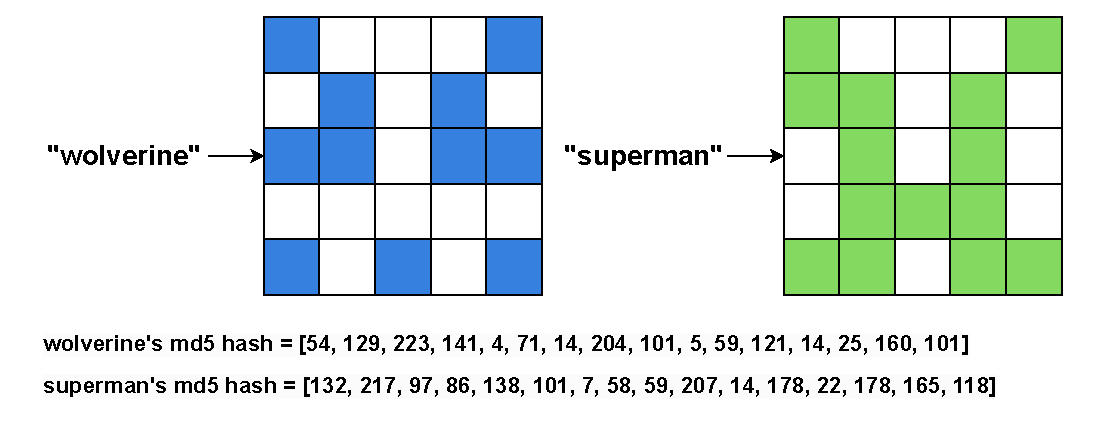
\includegraphics[width=\linewidth]{../../assets/avatar-example.pdf}
\end{figure}
\vspace{-10pt}
The 128-bit MD5 hash is split into 16 integers (0–255), each encoding color or grid placement.  
These values define the avatar’s pattern and symmetry, ensuring every input yields a unique, consistent design.


\end{frame}

\subsection{Avatar Pipeline}

\begin{frame}[fragile]{Avatar Pipeline}
\begin{figure}
  \centering
  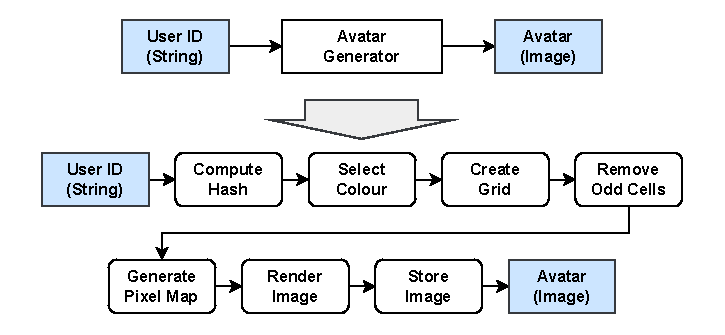
\includegraphics[width=.88\linewidth]{../../assets/avatar-pipeline.pdf}
\end{figure}
Input text is hashed (MD5, 128-bit/16 bytes) and drives color and layout. Functions run sequentially to transform data into a rendered PNG image.
\end{frame}

\begin{frame}[fragile]{Pipeline Code}
\vspace{20pt}
\begin{lstlisting}[language=Elixir]
compute_hash
|> select_color
|> create_grid
|> remove_odd_cells
|> generate_pixel_map
|> render_image
|> store_image
\end{lstlisting}

\small
\textbf{compute\_hash}: MD5 → 16 integers (0–255).  
\textbf{select\_color}: derives RGB from first bytes.  
\textbf{create\_grid}: builds 5×5 layout with symmetry.  
\textbf{remove\_odd\_cells}: keep even-valued cells.  
\textbf{generate\_pixel\_map}: map cells to coordinates.  
\textbf{render\_image}/\textbf{store\_image}: draw and save PNG.
\end{frame}

\subsection{Avatar Computation}

\begin{frame}[fragile]{Avatar Computation}
\begin{columns}[T,totalwidth=\textwidth]
  \begin{column}{0.4\textwidth}
    \small
    \begin{itemize}
      \item The avatar is generated as a \textbf{5×5 grid} image.
      \item \textbf{Columns 4 and 5 mirror columns 2 and 1}, creating symmetry and visual balance.
      \item \textbf{The first three columns} use integer values of the MD5 hash of the \texttt{username}.
      \item \textbf{Even} values fill colored cells; \textbf{odd} values remain white.
      \item \textbf{The first three hash bytes} define the RGB color used for the avatar.
    \end{itemize}
  \end{column}
\hfill
  \begin{column}{0.6\textwidth}
    \centering
    \begin{figure}
      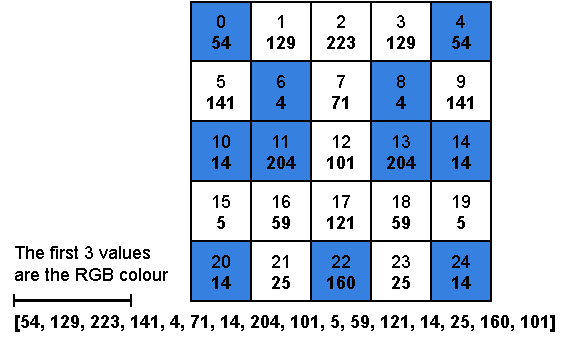
\includegraphics[width=\linewidth]{../../assets/avatar-computation.pdf}
      \caption{Hash integers, mirroring, and RGB mapping.}
    \end{figure}
  \end{column}
\end{columns}
\end{frame}

\section{Code Skeleton}
\begin{frame}[fragile]{Avatar Generator Code Skeleton}
\vspace{20pt}
\small
This code defines the main structure of the \texttt{AvatarGenerator} module in Elixir.  
Each function represents a stage in the avatar creation process — from hashing input data to generating and storing the final image.  
The modular design makes the pipeline readable, maintainable, and easy to extend. Keseluruhan Kode \texttt{src/avatar.ex}.

\begin{columns}[T,totalwidth=\textwidth]
  \begin{column}{0.48\textwidth}
    \begin{lstlisting}[language=Elixir, basicstyle=\ttfamily\scriptsize, firstnumber=1]
defmodule AvatarGenerator do
  use Application

  def generate(input) do
  end

  def compute_hash(input) do
  end

  def select_color(%Avatar.Image{
    hash: [r, g, b | _tail]} = image) do
  end
    \end{lstlisting}
  \end{column}

  \begin{column}{0.48\textwidth}
    \begin{lstlisting}[language=Elixir, basicstyle=\ttfamily\scriptsize, firstnumber=13]
  def create_grid(%Avatar.Image{
    hash: hash} = image) do
  end

  def reflect_row(row) do
  end

  def resize_list(list) do
  end

  def start(_type, _args) do
  end
end
    \end{lstlisting}
  \end{column}
\end{columns}
\end{frame}

\section{Image Structure Definition}
\begin{frame}[fragile]{Image Structure Definition}
\vspace{20pt}
\small
\begin{itemize}
  \item The \texttt{Avatar.Image} module defines a simple data structure used throughout the avatar generation process.
  \item It stores the computed MD5 hash and the selected RGB color, serving as a container for passing data between functions.
  \item The keyword \texttt{defstruct} in Elixir defines a structure (similar to a record or lightweight object) with named fields and default values.
  \item This enables the creation of consistent, easily managed data instances that can be passed and modified within the program.
\end{itemize}

\begin{lstlisting}[language=Elixir, caption={Definition of src/image.ex}, basicstyle=\ttfamily\small]
defmodule Avatar.Image do
  defstruct hash: nil, color: nil
end
\end{lstlisting}
\end{frame}



\section{Module Structure}

\begin{frame}[fragile]{Module Structure}
\vspace{20pt}
\small
The program is organized into two main modules, each serving a specific role in the avatar generation process:

\begin{itemize}
  \item \textbf{Avatar.Image}:  
  Defines a structured data type (\texttt{defstruct}) to store avatar-related information, including the MD5 hash and the RGB color used for rendering.

  \item \textbf{AvatarGenerator}:  
  Serves as the core logic module responsible for computing the hash, selecting colors, generating the symmetric grid, and producing the final avatar image.
\end{itemize}

Together, these modules separate data representation from processing logic, making the program modular, reusable, and easier to maintain.
\end{frame}

\section{The Avatar Image Structure}
\begin{frame}[fragile]{Defining the Avatar Image Structure}
\vspace{10pt}
\small
\begin{columns}[T,totalwidth=\textwidth]
  \begin{column}{0.5\textwidth}
    \begin{itemize}
      \item The \texttt{Avatar.Image} module defines a structure to store avatar-related data.
      \item It holds two main attributes:
      \begin{itemize}
        \item \texttt{hash} — stores the MD5 hash generated from the input string.
        \item \texttt{color} — stores the RGB color derived from the hash values.
      \end{itemize}
      \item The \texttt{defstruct} keyword defines these fields with default values of \texttt{nil}.
      \item This structure ensures consistent data handling during the avatar generation process.
    \end{itemize}
  \end{column}

  \begin{column}{0.4\textwidth}
    \begin{lstlisting}[language=Elixir, 
      caption={Defining the Avatar Image structure in \texttt{lib/image.ex}}, 
      basicstyle=\ttfamily\small]
defmodule Avatar.Image do
  defstruct hash: nil, color: nil
end
    \end{lstlisting}
  \end{column}
\end{columns}
\end{frame}


\section{Avatar Generation Module}
\begin{frame}[fragile]{Avatar Generator Module}
\vspace{10pt}
\begin{columns}[T,totalwidth=\textwidth]
  \begin{column}{0.52\textwidth}
    \small
    \begin{itemize}
      \item The \texttt{AvatarGenerator} module acts as the main logic controller for creating avatars.
      \item It uses the \texttt{Application} behavior, which enables defining the \texttt{start/2} function to initialize the app.
      \item The module coordinates the full workflow:
      \begin{itemize}
        \item computing hashes,
        \item selecting colors,
        \item generating grids,
        \item rendering and saving the final image.
      \end{itemize}
      \item It serves as the core engine combining helper functions into a structured, functional pipeline.
    \end{itemize}
  \end{column}

  \begin{column}{0.45\textwidth}
    \begin{lstlisting}[language=Elixir, 
      caption={Definition of the Avatar Generator module in \texttt{lib/avatar.ex}}, 
      basicstyle=\ttfamily\small]
defmodule AvatarGenerator do
  use Application
    \end{lstlisting}
  \end{column}
\end{columns}
\end{frame}

\section{Avatar Generation Function}
\begin{frame}[fragile]{Avatar Generation Function}
\vspace{10pt}
\begin{columns}[T,totalwidth=\textwidth]
  \begin{column}{0.52\textwidth}
    \small
    \begin{itemize}
      \item The \texttt{generate/1} function is the main entry point for creating an avatar.
      \item It accepts a string \texttt{input} (e.g., a username) and performs:
      \begin{itemize}
        \item hash computation using MD5,
        \item color selection based on hash values,
        \item grid creation for avatar visualization.
      \end{itemize}
      \item The Elixir pipeline operator (\texttt{|>}) passes results between functions,
      ensuring a clear and functional data flow.
    \end{itemize}
  \end{column}

  \begin{column}{0.46\textwidth}
    \begin{lstlisting}[language=Elixir, 
      caption={Main function for generating avatars}, 
      basicstyle=\ttfamily\small]
def generate(input) do
  input
  |> compute_hash
  |> select_color
  |> create_grid
end
    \end{lstlisting}
  \end{column}
\end{columns}
\end{frame}

\section{Compute the Hash}
\begin{frame}[fragile]{Computing the Hash}
\vspace{10pt}
\small
\begin{columns}[T,totalwidth=\textwidth]
  \begin{column}{0.52\textwidth}
    \begin{itemize}
      \item The \texttt{compute\_hash/1} function generates an MD5 hash from the given input string.
      \item It uses the built-in \texttt{:crypto} module to produce a 128-bit binary hash.
      \item The hash is then converted into a list of integers (0–255) using \texttt{:binary.bin\_to\_list/1}.
      \item The \texttt{resize\_list/1} helper ensures the list length is a multiple of three, aligning it with the RGB grouping used later.
      \item The resulting hash list is stored in a new \texttt{\%Avatar.Image\{\}} struct.
    \end{itemize}
  \end{column}

  \begin{column}{0.43\textwidth}
    \begin{lstlisting}[language=Elixir, 
      caption={Computing the hash from the input string}, 
      basicstyle=\ttfamily\footnotesize]
def compute_hash(input) do
  hash =
    :crypto.hash(:md5, input)
    |> :binary.bin_to_list()
    |> resize_list

  IO.inspect(hash)
  %Avatar.Image{hash: hash}
end
    \end{lstlisting}
  \end{column}
\end{columns}
\end{frame}

\section{Resizing Hash List}
\begin{frame}[fragile]{Helper Function: Resizing the Hash List}
\small
\begin{itemize}
  \item The \texttt{resize\_list/1} function ensures the hash list length is a multiple of three for proper RGB grouping and grid layout.
  \item \texttt{length(list)} counts the elements, and \texttt{div(length(list), 3) * 3} calculates the nearest lower multiple of three.
  \item \texttt{Enum.take(list, full\_chunks\_count)} keeps only that portion, trimming excess elements for a balanced, symmetric avatar grid.
\end{itemize}

\begin{lstlisting}[language=Elixir, basicstyle=\ttfamily\small]
def resize_list(list) do
  full_chunks_count = div(length(list), 3) * 3
  Enum.take(list, full_chunks_count)
end
\end{lstlisting}
\end{frame}

\section{Selecting Avatar Color}
\begin{frame}[fragile]{Selecting the Avatar Color}
\small
\begin{itemize}
  \item The \texttt{select\_color/1} function extracts the first three elements of the hash list.
  \item These values represent the red (\texttt{r}), green (\texttt{g}), and blue (\texttt{b}) components of the avatar’s color.
  \item The color is stored as an RGB tuple \texttt{\{r, g, b\}} inside the \texttt{Avatar.Image} struct.
  \item This ensures that each input string produces a unique and consistent color scheme.
\end{itemize}

\begin{lstlisting}[language=Elixir, basicstyle=\ttfamily\footnotesize]
def select_color(%Avatar.Image{hash: [r, g, b | _tail]} = image) do
  %Avatar.Image{image | color: {r, g, b}}
end
\end{lstlisting}
\end{frame}

\section{Creating the Avatar Grid}
\begin{frame}[fragile]{Creating the Avatar Grid}
\vspace{20pt}
\begin{itemize}
  \item The \texttt{create\_grid/1} function converts the hash list into a symmetric grid pattern. 
	\item It splits the hash into rows of three elements using \texttt{Enum.chunk\_every(3)}.
  \item Each row is mirrored with \texttt{reflect\_row/1} to create horizontal symmetry.
  \item The resulting list of rows is flattened and indexed with \texttt{Enum.with\_index/1}. 
\item This indexed grid defines the structure and position of each cell in the avatar.
\end{itemize}

\begin{lstlisting}[language=Elixir, basicstyle=\ttfamily\small]
def create_grid(%Avatar.Image{hash: hash} = image) do
  hash
  |> Enum.chunk_every(3)
  |> Enum.map(&reflect_row/1)
  |> List.flatten
  |> Enum.with_index
end
\end{lstlisting}
\end{frame}

\section{Reflecting Row Symmetry}
\begin{frame}[fragile]{Reflecting Rows for Symmetry}
\small
\begin{itemize}
  \item The helper function \texttt{reflect\_row/1} ensures horizontal symmetry in the avatar grid.
  \item It takes a row of three elements and mirrors the first two values in reverse order.
  \item This produces a five-element row, creating a balanced, symmetric pattern.
  \item The mirrored layout contributes to the visual harmony of the generated avatar.
\end{itemize}

\begin{lstlisting}[language=Elixir, basicstyle=\ttfamily\small]
def reflect_row(row) do
  [first, second | _tail] = row
  row ++ [second, first]
end
\end{lstlisting}
\end{frame}

\section{Starting the Application}
\begin{frame}[fragile]{Starting the Application}
\small
\begin{itemize}
  \item The \texttt{start/2} function is automatically executed when the application launches.
  \item It calls \texttt{AvatarGenerator.generate("wolverine")} to create an avatar from the sample input.
  \item The resulting grid data structure is printed to the console using \texttt{IO.inspect/1}.
  \item The function returns \texttt{{:ok, self()}}, signaling successful startup and keeping the application process active.
\end{itemize}

\begin{lstlisting}[language=Elixir, basicstyle=\ttfamily\small]
def start(_type, _args) do
  result = AvatarGenerator.generate("wolverine")
  IO.inspect(result)
  {:ok, self()}
end
\end{lstlisting}
\end{frame}

\section{Running the Application}
\begin{frame}[fragile]{Running the Application}
\small
\begin{itemize}
  \item To run the application, the configuration in \texttt{mix.exs} must specify the starting module.
  \item This is done by adding the \texttt{mod} attribute inside the \texttt{application} function.
  \item Here, \texttt{AvatarGenerator} is defined as the main module that initializes the app on startup.
  \item The \texttt{extra\_applications} key includes default dependencies such as \texttt{:logger}.
\end{itemize}

\begin{lstlisting}[language=Elixir, basicstyle=\ttfamily\small]
def application do
  [
    extra_applications: [:logger],
    mod: {AvatarGenerator, []}
  ]
end
\end{lstlisting}
\end{frame}

\section{Conclusion}
\begin{frame}[fragile]{Conclusion}
\small
This chapter explained the implementation of an avatar generator using the Elixir programming language.  
The project utilizes:
\begin{itemize}
  \item the \texttt{:crypto} module to compute MD5 hashes,
  \item Elixir’s \texttt{struct} feature to store avatar data,
  \item and list operations to create a grid-based visual representation.
\end{itemize}
The application is managed through the \texttt{Application} behavior, enabling it to run as a standalone Elixir app.  
Overall, the design demonstrates modular, functional programming principles for generating unique, symmetric avatars.
\end{frame}


\end{document}
